\documentclass[border=10pt]{standalone}
\usepackage{tikz}
\usepackage[margin=1in]{geometry}
\usetikzlibrary{positioning, arrows.meta, decorations.pathmorphing, patterns, calc, shadows.blur}

\begin{document}
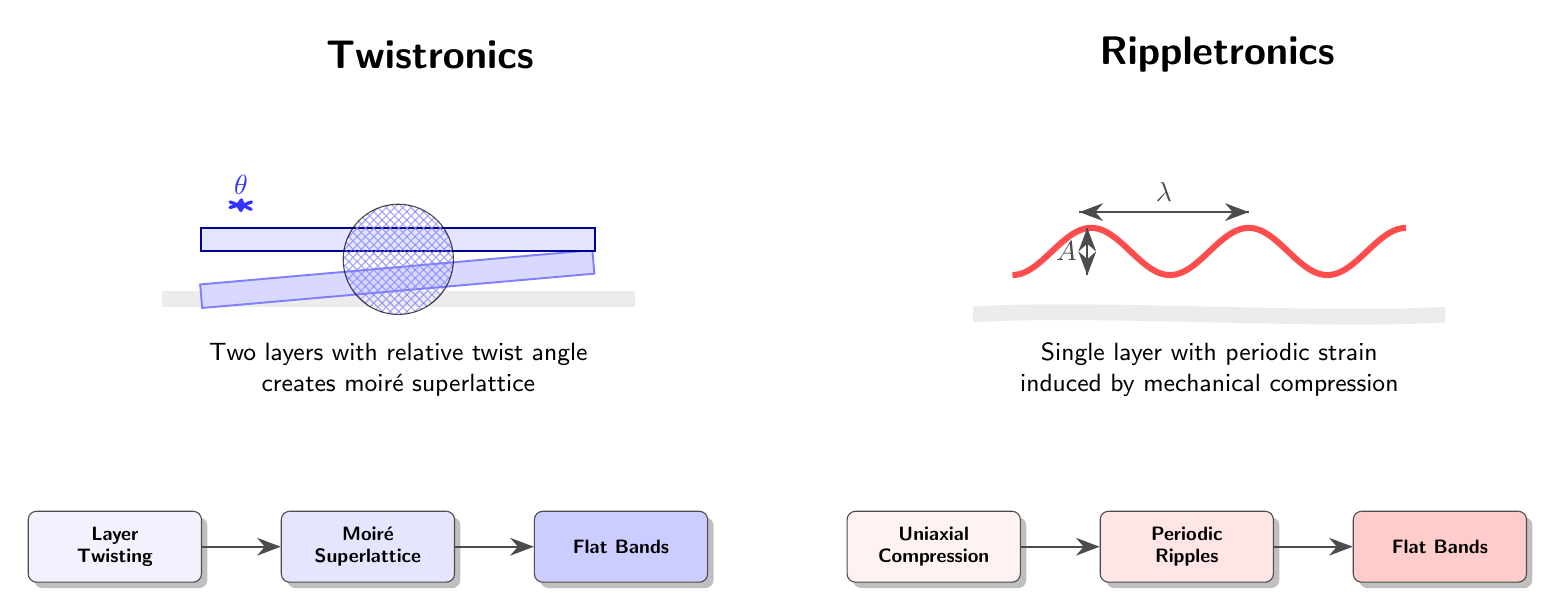
\begin{tikzpicture}[
    font=\sffamily,
    panel/.style={draw=black!30, fill=white, rounded corners=3pt, inner sep=10pt, drop shadow},
    label/.style={font=\sffamily\small, align=center},
    flownode/.style={
        draw=black!70, fill=white, drop shadow,
        rounded corners=3pt,
        minimum height=0.9cm, minimum width=2.2cm,
        align=center, font=\sffamily\scriptsize\bfseries, text=black
    },
    arrow/.style={-{Stealth[length=3mm]}, line width=0.8pt, color=black!70}
]

% Titles
\node at (-5,5) {\Large\bfseries Twistronics};
\node at (5,5) {\Large\bfseries Rippletronics};

%%%%%%%%%%%%%%%%%%%%%
% Twistronics Diagram
%%%%%%%%%%%%%%%%%%%%%
\begin{scope}[shift={(-5.4,2.5)}]
    \fill[gray!15] (-3,-0.5) rectangle (3,-0.7);

    \path[fill=blue!15, draw=blue!50, line width=0.7pt, rotate around={5:(0,-0.5)}] 
        (-2.5,-0.5) rectangle (2.5,-0.2);
    \path[fill=blue!10, draw=blue!60!black, line width=0.7pt] 
        (-2.5,0) rectangle (2.5,0.3);

    \draw[pattern=crosshatch, pattern color=blue!50, opacity=0.7] (0,-0.1) circle (0.7);

    \draw[<->, very thick, blue!80] (-2,0.5) arc (180:175:2) node[midway, above] {$\theta$};

    \node[label, text width=5cm] at (0,-1.5) 
         {Two layers with relative twist angle\\creates moiré superlattice};
\end{scope}

%%%%%%%%%%%%%%%%%%%%%
% Rippletronics Diagram with improved sine ripple
%%%%%%%%%%%%%%%%%%%%%
\begin{scope}[shift={(4.9,2.5)}]
    % Substrate
    \fill[gray!15]
        (-3,-0.7) .. controls (-1.5,-0.6) and (1.5,-0.8) .. (3,-0.7)
        -- (3,-0.9) .. controls (1.5,-1.0) and (-1.5,-0.8) .. (-3,-0.9) -- cycle;

    % Sine-like ripple (clean symmetric)
    \draw[red!70, line width=2.2pt]
        plot[domain=-2.5:2.5, samples=100, smooth] 
        (\x,{0.3*sin(180*\x)});

    \draw[arrow=red!80] (-1.65,0.5) -- (0.5,0.5) node[midway, above] {$\lambda$};
    \draw[arrow=red!80] (0.5,0.5) -- (-1.65,0.5);

    \draw[arrow=red!80] (-1.55,-0.3) -- (-1.55,0.3) node[midway, left] {$A$};
    \draw[arrow=red!80] (-1.55,0.3) -- (-1.55,-0.3);
    
    \node[label, text width=5cm] at (0,-1.5)
         {Single layer with periodic strain\\induced by mechanical compression};
\end{scope}

%%%%%%%%%%%%%%%%%%%%%
% Twistronics Flow (compact horizontal)
%%%%%%%%%%%%%%%%%%%%%
\begin{scope}[shift={(-9,-1.25)}, node distance=1cm]
    \node[flownode, fill=blue!5] (twist) {Layer\\Twisting};
    \node[flownode, fill=blue!10, right=of twist] (moire) {Moiré\\Superlattice};
    \node[flownode, fill=blue!20, right=of moire] (flatbandsT) {Flat Bands};

    \draw[arrow] (twist) -- (moire);
    \draw[arrow] (moire) -- (flatbandsT);
\end{scope}

%%%%%%%%%%%%%%%%%%%%%
% Rippletronics Flow (compact horizontal)
%%%%%%%%%%%%%%%%%%%%%
\begin{scope}[shift={(1.4,-1.25)}, node distance=1cm]
    \node[flownode, fill=red!5] (comp) {Uniaxial\\Compression};
    \node[flownode, fill=red!10, right=of comp] (ripple) {Periodic\\Ripples};
    \node[flownode, fill=red!20, right=of ripple] (flatbandsR) {Flat Bands};

    \draw[arrow] (comp) -- (ripple);
    \draw[arrow] (ripple) -- (flatbandsR);
\end{scope}

\end{tikzpicture}
\end{document}
